\documentclass[a4paper,12pt]{article} 
\usepackage[T2A]{fontenc}			
\usepackage[utf8]{inputenc}			
\usepackage[english,russian]{babel}	
\usepackage{amsmath,amsfonts,amssymb,amsthm,mathrsfs,mathtools} 
\usepackage{cancel}
\usepackage{multirow}
\usepackage[colorlinks, linkcolor = blue]{hyperref}
\usepackage{upgreek}\usepackage[left=2cm,right=2cm,top=2cm,bottom=3cm,bindingoffset=0cm]{geometry}
\usepackage{graphicx,wrapfig,subfig}
\usepackage{xcolor}
\graphicspath{ {./images/} }

\author{Толстикова М.С.\\
Группа Б04-205}

\title{\textbf{3.2.5 (4.б). Свободные и вынужденные колебания в электрическом контуре.}}

\date{14 сентября 2023 г.}

\begin{document}
\maketitle

\leftskip=1cm \rightskip=1cm

\textbf{Цель работы}: исследования свободных и вынужденных колебаний в колебательном контуре.

\textbf{В работе используются}: осциллограф АКТАКОМ ADS-6142H, генератор сигналов специальной формы АКИП-3409/4, магазин сопротивления МСР-60, магазин ёмкости Р5025, магазин индуктивности Р567 типа МИСП, соединительная коробка с шунтирующей емкостью, соединительные одножильные и коаксиальные провода.

\leftskip=0cm \rightskip=0cm

\section*{1. Теоритические сведения.}

Рассмотрим электрический контур, состоящий из последовательно соединённых конденстора $C$, катушки индуктивности $L$ и резистора $R$. Обозначим разность потенциалов на конденсаторе $U_C$, а ток, текущий в контуре, через $I$. Второе правило Кирхгофа:

\begin{equation}
L \dfrac{d^2I}{dt^2}+R\dfrac{dI}{dt}+\dfrac{I}{C}=0.
\end{equation}

Вводя обозначения $\gamma = \dfrac{R}{2L}$, $\omega_0^2=\dfrac{1}{LC}$, получим уравнение

\begin{equation}
\ddot{I}+2\gamma\dot{I}+\omega_0^2I=0.
\end{equation}

Его решение в общем виде:

\begin{equation}
I = -\dfrac{U_0}{L\kappa}e^{-\gamma t}\text{sh}(\kappa t), 
\end{equation}

где $\kappa = \sqrt{\gamma^2 - \omega_0^2}$, $U_0 = U_C$ -- начальное напряжение на конденсаторе.

 В случае, когда $\gamma < \omega_0$, имеем $\kappa = i\omega$, где $\omega = \sqrt{\omega_0^2 - \gamma^2}$ -- \textit{частоты свободных (собственных) колебаний}. Тогда ток
 
 \begin{equation}
 I = -\dfrac{U_0}{L\omega}e^{-\gamma t}\sin(\omega t)
 \end{equation}
 
 затухает и имеет колебательный характер. Величина $\gamma$ определяет затухание колебаний: $\gamma = \dfrac{1}{\tau}$, где $\tau$ -- время затухание амплитуды в $e$ раз.
 
Формулы для напряжения на кондесаторе и тока в цепи можно переписать иначе:

\begin{equation}
\begin{array}{c}
U_C = U_0 \dfrac{\omega_0}{\omega}e^{-\gamma t} \cos(\omega t - \theta),\\
\\
I = -\dfrac{U_0}{L}e^{-\gamma t} \cos(\omega t - \theta).
\end{array}
\end{equation}

В случае $\gamma > \omega_0$, формулы для тока и напряжения на конденсаторе имеют следующий вид:
$$
\begin{array}{c}
I = -\dfrac{U_0}{L\kappa}e^{-\gamma t}\text{sh}(\kappa t),\\
\\
U_C = U_0 e^{-\gamma t}\left( \dfrac{\gamma}{\kappa}\text{sh}(\kappa t) + \text{ch}(\kappa t) \right).
\end{array}
$$
Процесс в этом случае не является колебательным, его называют апериодическим. Режим, соответствующий $\gamma = \omega_0$, называются \textit{критическим}. В этом случае предельный переход $\omega \rightarrow 0$ в $(5)$ даст 
$$
\begin{array}{c}
I = -\dfrac{U_0}{L}te^{-\gamma t},\\
\\
U_C=U_0 e^{-\gamma t}(1+\gamma t).
\end{array}
$$
Сопротивление в этом случае 
\begin{equation}
R_{\text{кр}}= 2 \sqrt{\dfrac{L}{C}}
\end{equation}
называется \textit{критическим сопротивлением} контура.\\
\textit{Добротность} контура по определению 
$$
Q = 2\pi \dfrac{W}{\Delta W},
$$ 
где $W$ -- запасённая энергия, $\Delta W$ -- потери за период. Тогда
\begin{equation}
Q = 2\pi\dfrac{CU_0^2/2 \cdot e^{-2\gamma t}}{CU_0^2/2 \cdot (e^{-2\gamma t} - e^{-2\gamma (T+t)})}=\dfrac{\pi}{\gamma T}=\dfrac{1}{R}\sqrt{\dfrac{L}{C}}.
\end{equation}
\textit{Логарифмическим декрементом затухания} называются число
\begin{equation}
\Theta = \text{ln}\dfrac{U_k}{U_{k+1}}=\text{ln} e^{\gamma T}=\gamma T.
\end{equation}
или 
\begin{equation}
\Theta = \dfrac{1}{n} \text{ln}\dfrac{U_k}{U_{k+n}}.
\end{equation}

\newpage

\section*{2. Экспериментальная установка.}

Колебательный контур состоит из постоянной индуктивности $L$ с активным сопротивлением $RL$, переменной емкости $C$ и сопротивления $R$. 
Картина колебаний напряжения на емкости наблюдается на экране двухканального осциллографа. Для возбуждения затухающих колебаний используется генератор сигналов специальной формы.
Сигнал с генератора поступает через конденсатор C1 на вход колебательного контура. Данная емкость необходима чтобы выходной импеданс генератора был много меньше импеданса колебательного контура и не влиял на процессы, проходящие в контуре. 

\begin{figure}[h]
    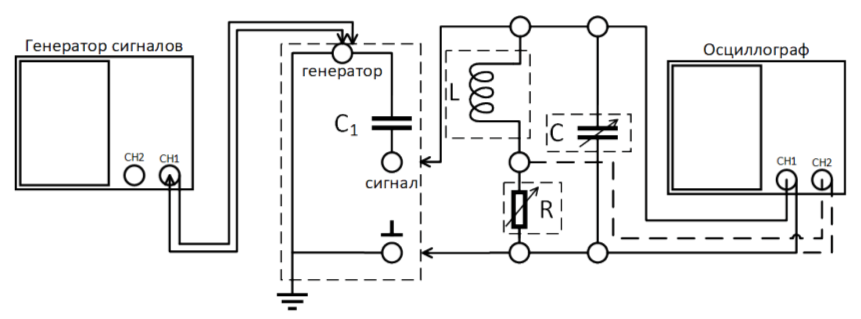
\includegraphics[scale=0.5]{ustanovka.png}
    \centering
    \caption{ Схема установки для исследования вынужденных колебаний}
\end{figure}

При изучении свободно затухающих колебаний генератор специальных сигналов на вход колебательного контура подает периодические короткие импульсы, которые заряжают конденсатор $C$. За время между
последовательными импульсами происходит разрядка конденсатора через резистор и катушку индуктивности. Напряжение на конденсаторе $U_C$ поступает на вход канала 1(X) электронного осциллографа. Для наблюдения фазовой картины затухающих колебаний на канал 2(Y) подается напряжение с резистора $R$ (пунктирная линия на
схеме установки), которое пропорционально току $I$ ($I\propto dU_C/dt$).
При изучении возбужденных колебаний на вход колебательного контура подается
синусоидальный сигнал. С помощью осциллографа возможно измерить зависимость
амплитуды возбужденных колебаний в зависимости от частоты внешнего сигнала,
из которого возможно определить добротность колебательного контура. Альтернативным способом расчета добротности контура является определение декремента
затухания по картине установления возбужденных колебаний. В этом случае генератор сигналов используется для подачи цугов синусоидальной формы.


\section*{3. Ход работы}

\subsection*{3.1. Измерение свободных колебаний.}

Устанавливаем на магазине сопротивлений величину $R = 0$ Ом,на магазине индуктивностей $L = 100$ мГн (это значение остается постоянным), на магазине емкостей величину $C = 0$ мкФ.

Найдем минимальное значение емкости контура $C_0$, благодаря которому в контуре реализуются свободные колебания. При этом затухание обеспечивается наличием активного сопротивления в магазине индуктивностей $R_L$.\\
Период колебаний: $T = 66,4$ мкс
$$
C_0=\frac{T^2}{4\pi^2L}=1\text{нФ}
$$

\begin{table}[!ht]
    \centering
    \begin{tabular}{|c|c|c|}
    \hline
        С, мкф & $T_{theor}$, мкс & $T_{exp}$, мкс \\ \hline
        0,002 & 89 & 93 \\ \hline
        0,003 & 109 & 112 \\ \hline
        0,005 & 140 & 143 \\ \hline
        0,007 & 166 & 168 \\ \hline
        0,009 & 188 & 191 \\ \hline
        0,01 & 199 & 200 \\ \hline
    \end{tabular}
\caption{Теоритически и экспериментально полученные значения периодов.}
\end{table}

\begin{figure}[h]
    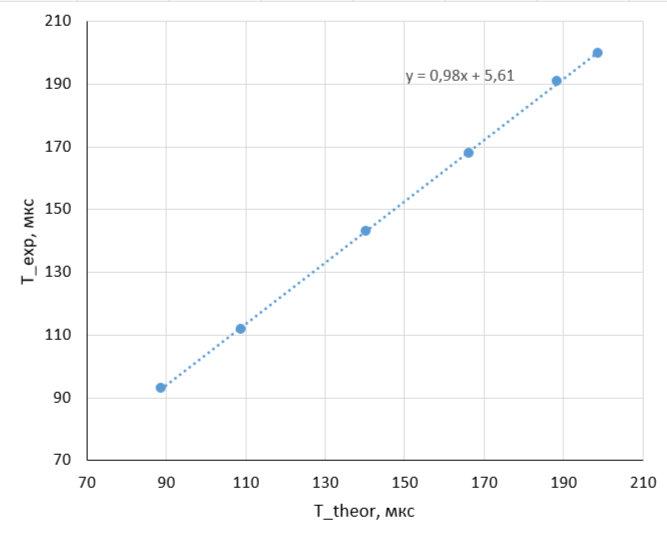
\includegraphics[scale=0.5]{1.png}
    \centering
    \caption{График $T_{exp}=f(T_{theor})$}
\end{figure}

\subsection*{3.2. Логарифмический декремент затухания и сопротивление контура.}

$L = 100$ мГн, рассчитаем емкость $C^*$ при которой собственная частота колебаний\\ $\nu_0 = \frac{1}{2\pi\sqrt{LC}}$ составляет 6.5 кГц.
$$
R_{cr} = 2\sqrt{L/C^*} = 8 \text{ кОм}
$$
В эксперименте получилось $R_{cr} = 5,8$ кОм
\newpage
\begin{table}[!ht]
    \centering
    \begin{tabular}{|l|l|l|l|l|l|}
    \hline
        $R/R_{cr}$ & $R$, Ом & n & $U_{m}$, В & $U_{m+n}$, В & $\Theta$ \\ \hline
        0,05 & 290 & 4 & 8,92 & 2,96 & 0,28 \\ \hline
        0,086 & 500 & 4 & 8,56 & 1,56 & 0,43 \\ \hline
        0,12 & 700 & 4 & 8,24 & 0,84 & 0,57 \\ \hline
        0,155 & 900 & 4 & 8 & 0,52 & 0,68 \\ \hline
        0,19 & 1100 & 3 & 7,8 & 0,6 & 0,85 \\ \hline
        0,22 & 1300 & 2 & 7,64 & 0,96 & 1,04 \\ \hline
        0,25 & 1450 & 2 & 7,32 & 0,8 & 1,11 \\ \hline
    \end{tabular}
\caption{Расчет декремента затухания}
\end{table}

$\Theta_{min} = 0,28$, $Q = 11,21$

$\Theta_{max} = 1,11$, $Q = 2,83$

$1/\Theta^2 = X, 1/R_\Sigma^2 = Y$



$k = \Delta Y/\Delta X = (14,6\pm 0,2)*10^5$
$$
R_{cr} = 2\pi\sqrt{\Delta Y/\Delta X} = 7,59\pm0,05 \text{кОм}
$$
\subsection*{3.3. Декремент затухания на фазовой плоскости.}
На фазовой плоскости:\\
1) При $R_1$ = 290 Ом 
$$
\Theta_1 = \frac{1}{n} \ln{x_m/x_{m+n}} = 0,29,
Q_1 =\pi/\Theta = 10,83
$$
2) При $R_2$ = 1450 Ом 

$$
\Theta_2 = \frac{1}{n} \ln{x_m/x_{m+n}} = 1,1,  
Q_2 = \pi/\Theta = 2,85
$$

\subsection*{3.4. Теоритический расчет.} 
Рассчитаем добротность теоритически через $R$, $L$, $C$.
$$
Q = \dfrac{1}{R}\sqrt{\dfrac{L}{C}}.
$$
1) При R = 290 Ом 
$$
Q_1 = 12,01
$$
2) При R = 1450 Ом 
$$
Q_2 = 2,72
$$

\subsection*{3.5. Добротность через АЧХ.}

$\nu_{res} = 6430$ Гц, при этом $U_0 = 135$ В. Проводим измерения для $R_1$ и $R_2$.

Для $R_1$: $2\Delta\Omega = 0,09$, 

$$
Q_1 = \frac{\omega_0}{2\Delta\Omega}=11,11
$$

Для $R_2$ мы не можем точно определить $2\Delta\Omega$ по ширине резонансной кривой, поэтому оценим ее шириной кривой от точки на уровне $1/\sqrt{2}$ до максимума, умноженной на 2.\\
$2\Delta\Omega = 0,15$, 

$$
Q_2 = 3,33
$$

\begin{figure}[h]
    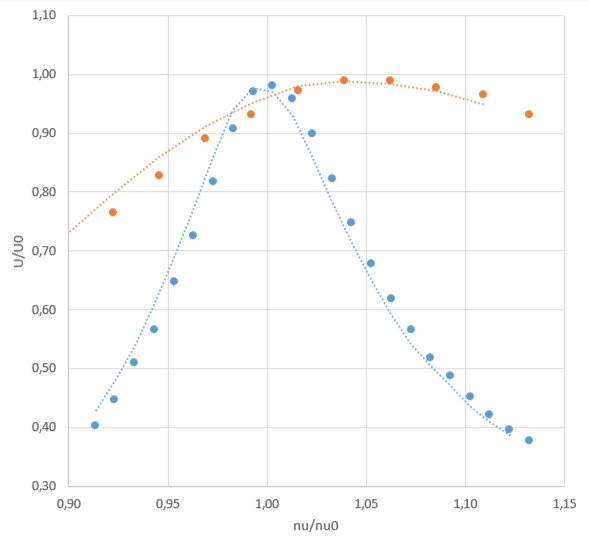
\includegraphics[scale=0.6]{3.png}
    \centering
    \caption{График резонансных кривых}
\end{figure}

\subsection*{3.6. Добротность через ФЧХ.}

Определим добротность контура по ФЧХ.

Для $R_1$:\\
По графику определяем $\Delta\omega = 3700$ Ом, 

$$
Q_1 = \frac{\omega_0}{\Delta\omega} = 10,9
$$

\begin{figure}[h]
    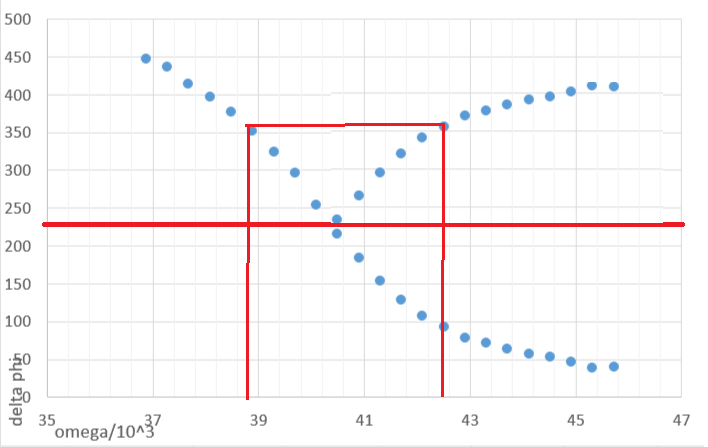
\includegraphics[scale=0.6]{4.png}
    \centering
    \caption{ФЧХ для $R_1$}
\end{figure}

Для $R_2$ не хватает данных, чтобы найти добротность через ФЧХ.

\newpage

\begin{figure}[h]
    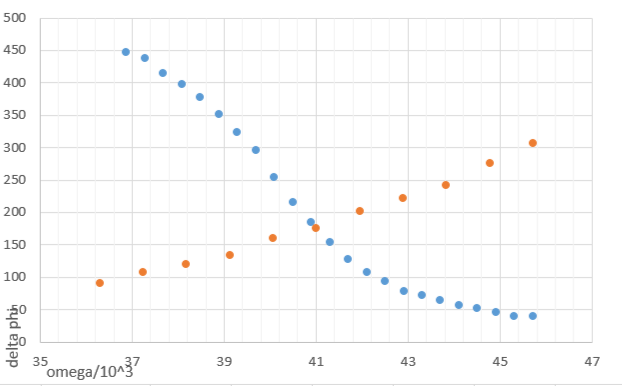
\includegraphics[scale=0.6]{5.png}
    \centering
    \caption{ФЧХ для $R_1$ и $R_2$}
\end{figure}

\subsection*{3.7. Добротность по скорости нарастания и затухания колебаний.}

Для $R_1$: $U_0 = 256$ В\\
При нарастании амплитуды декремент затухания считаем по формуле:
$$
\Theta = \frac{1}{n}\ln{\frac{U_0-U_k}{U_0-U_{k+n}}}
$$
\begin{table}[!ht]
    \centering
    \begin{tabular}{|l|l|l|l|}
    \hline
        n & U\_k & U\_k+n & Theta \\ \hline
        4 & 34 & 99 & 0,294 \\ \hline
        3 & 57 & 99 & 0,298 \\ \hline
        3 & 34 & 89 & 0,293 \\ \hline
        2 & 34 & 76 & 0,296 \\ \hline
        2 & 57 & 89 & 0,300 \\ \hline
    \end{tabular}
\end{table}
$$
\Theta_1 = 0,296 \pm 0,006
$$
$$
Q_1 = 10,6 \pm 0,
$$
При затухании амплитуды декремент затухания считаем по формуле:
$$
\Theta_1 = \frac{1}{n}\ln{\frac{U_k}{U_{k+n}}}
$$
\begin{table}[!ht]
    \centering
    \begin{tabular}{|l|l|l|l|}
    \hline
        n & Uk & Uk+m & Theta \\ \hline
        4 & 94 & 30 & 0,286 \\ \hline
        3 & 94 & 40 & 0,285 \\ \hline
        3 & 71 & 30 & 0,287 \\ \hline
        2 & 71 & 40 & 0,287 \\ \hline
        2 & 94 & 53 & 0,287 \\ \hline
    \end{tabular}
\end{table}

$$
\Theta_1 = 0,286 \pm 0,006
$$
$$
Q_1 = 11 \pm 0,2
$$

Для $R_2$: $U_0 = 33,7$ В\\
При нарастании:
$$
\Theta_2 = \frac{1}{n}\ln{\frac{U_0-U_k}{U_0-U_{k+n}}} = \frac{1}{2}\ln{\frac{33,7-8,8}{33,7-30,8}} = 1,08\pm0,02
$$
$$
Q_2 = 2,9\pm0,1
$$

При затухании:
$$
\Theta_2 = \frac{1}{2}\ln{\frac{31,4}{3}} = 1,17\pm0,04
$$
$$
Q_2 = 2,7\pm0,1
$$

\section*{4.Вывод}

\begin{table}[!ht]
\begin{tabular}{|l|cll|llll|}
\hline
\multirow{2}{*}{R} & \multicolumn{3}{c|}{Свободные колебания}                                                                     & \multicolumn{4}{c|}{Вынужденные колебания}                                                                                                                                 \\ \cline{2-8} 
                   & \multicolumn{1}{c|}{$f(L, C, R)$} & \multicolumn{1}{l|}{$f(\Theta)$}                   & Спираль                  & \multicolumn{1}{l|}{АЧХ}                      & \multicolumn{1}{l|}{ФЧХ}                   & \multicolumn{1}{l|}{Нарастание}                  & Затухание                  \\ \hline
R1                 & \multicolumn{1}{c|}{$12\pm1$}      & \multicolumn{1}{l|}{$11,2\pm0,2$}  & $10\pm1$    & \multicolumn{1}{l|}{$11\pm1$}    & \multicolumn{1}{l|}{$11\pm1$} & \multicolumn{1}{l|}{$10,6 \pm 0,5$} & $11 \pm 0,2$  \\ \hline
R2                 & \multicolumn{1}{c|}{$2,7\pm0,2$}       & \multicolumn{1}{l|}{$2,83\pm0,06$} & $2,9\pm0,3$ & \multicolumn{1}{l|}{$3,3\pm0,4$} & \multicolumn{1}{l|}{}                      & \multicolumn{1}{l|}{$2,9\pm0,1$}  & $2,7\pm0,1$ \\ \hline
\end{tabular}
\end{table}

В пределах погрешностей все значения, кроме теоритических, совпадают. Самые точные методы измерения добротности - $f(\Theta)$ в свободных колебаниях и нарастание и затухание в вынужденных.
\end{document}